\documentclass[11pt,a4paper]{report}
\usepackage[textwidth=37em,vmargin=30mm]{geometry}
\usepackage{calc,xunicode,amsmath,amssymb,paralist,enumitem,tabu,booktabs,datetime2,xeCJK,xeCJKfntef,listings}
\usepackage{tocloft,fancyhdr,tcolorbox,xcolor,graphicx,eso-pic,xltxtra,xelatexemoji}

\newcommand{\envyear}[0]{2025}
\newcommand{\envdatestr}[0]{2025-05-02}
\newcommand{\envfinaldir}[0]{webdb/2025/20250502/final}

\usepackage[hidelinks]{hyperref}
\hypersetup{
    colorlinks=false,
    pdfpagemode=FullScreen,
    pdftitle={Web Digest - \envdatestr}
}

\setlength{\cftbeforechapskip}{10pt}
\renewcommand{\cftchapfont}{\rmfamily\bfseries\large\raggedright}
\setlength{\cftbeforesecskip}{2pt}
\renewcommand{\cftsecfont}{\sffamily\small\raggedright}

\setdefaultleftmargin{2em}{2em}{1em}{1em}{1em}{1em}

\usepackage{xeCJK,xeCJKfntef}
\xeCJKsetup{PunctStyle=plain,RubberPunctSkip=false,CJKglue=\strut\hskip 0pt plus 0.1em minus 0.05em,CJKecglue=\strut\hskip 0.22em plus 0.2em}
\XeTeXlinebreaklocale "zh"
\XeTeXlinebreakskip = 0pt


\setmainfont{Brygada 1918}
\setromanfont{Brygada 1918}
\setsansfont{IBM Plex Sans}
\setmonofont{JetBrains Mono NL}
\setCJKmainfont{Noto Serif CJK SC}
\setCJKromanfont{Noto Serif CJK SC}
\setCJKsansfont{Noto Sans CJK SC}
\setCJKmonofont{Noto Sans CJK SC}

\setlength{\parindent}{0pt}
\setlength{\parskip}{8pt}
\linespread{1.15}

\lstset{
	basicstyle=\ttfamily\footnotesize,
	numbersep=5pt,
	backgroundcolor=\color{black!5},
	showspaces=false,
	showstringspaces=false,
	showtabs=false,
	tabsize=2,
	captionpos=b,
	breaklines=true,
	breakatwhitespace=true,
	breakautoindent=true,
	linewidth=\textwidth
}






\newcommand{\coverpic}[2]{
    % argv: itemurl, authorname
    Cover photo by #2~~(\href{#1}{#1})
}
\newcommand{\makeheader}[0]{
    \begin{titlepage}
        % \newgeometry{hmargin=15mm,tmargin=21mm,bmargin=12mm}
        \begin{center}
            
            \rmfamily\scshape
            \fontspec{BaskervilleF}
            \fontspec{Old Standard}
            \fontsize{59pt}{70pt}\selectfont
            WEB\hfill DIGEST
            
            \vfill
            % \vskip 30pt
            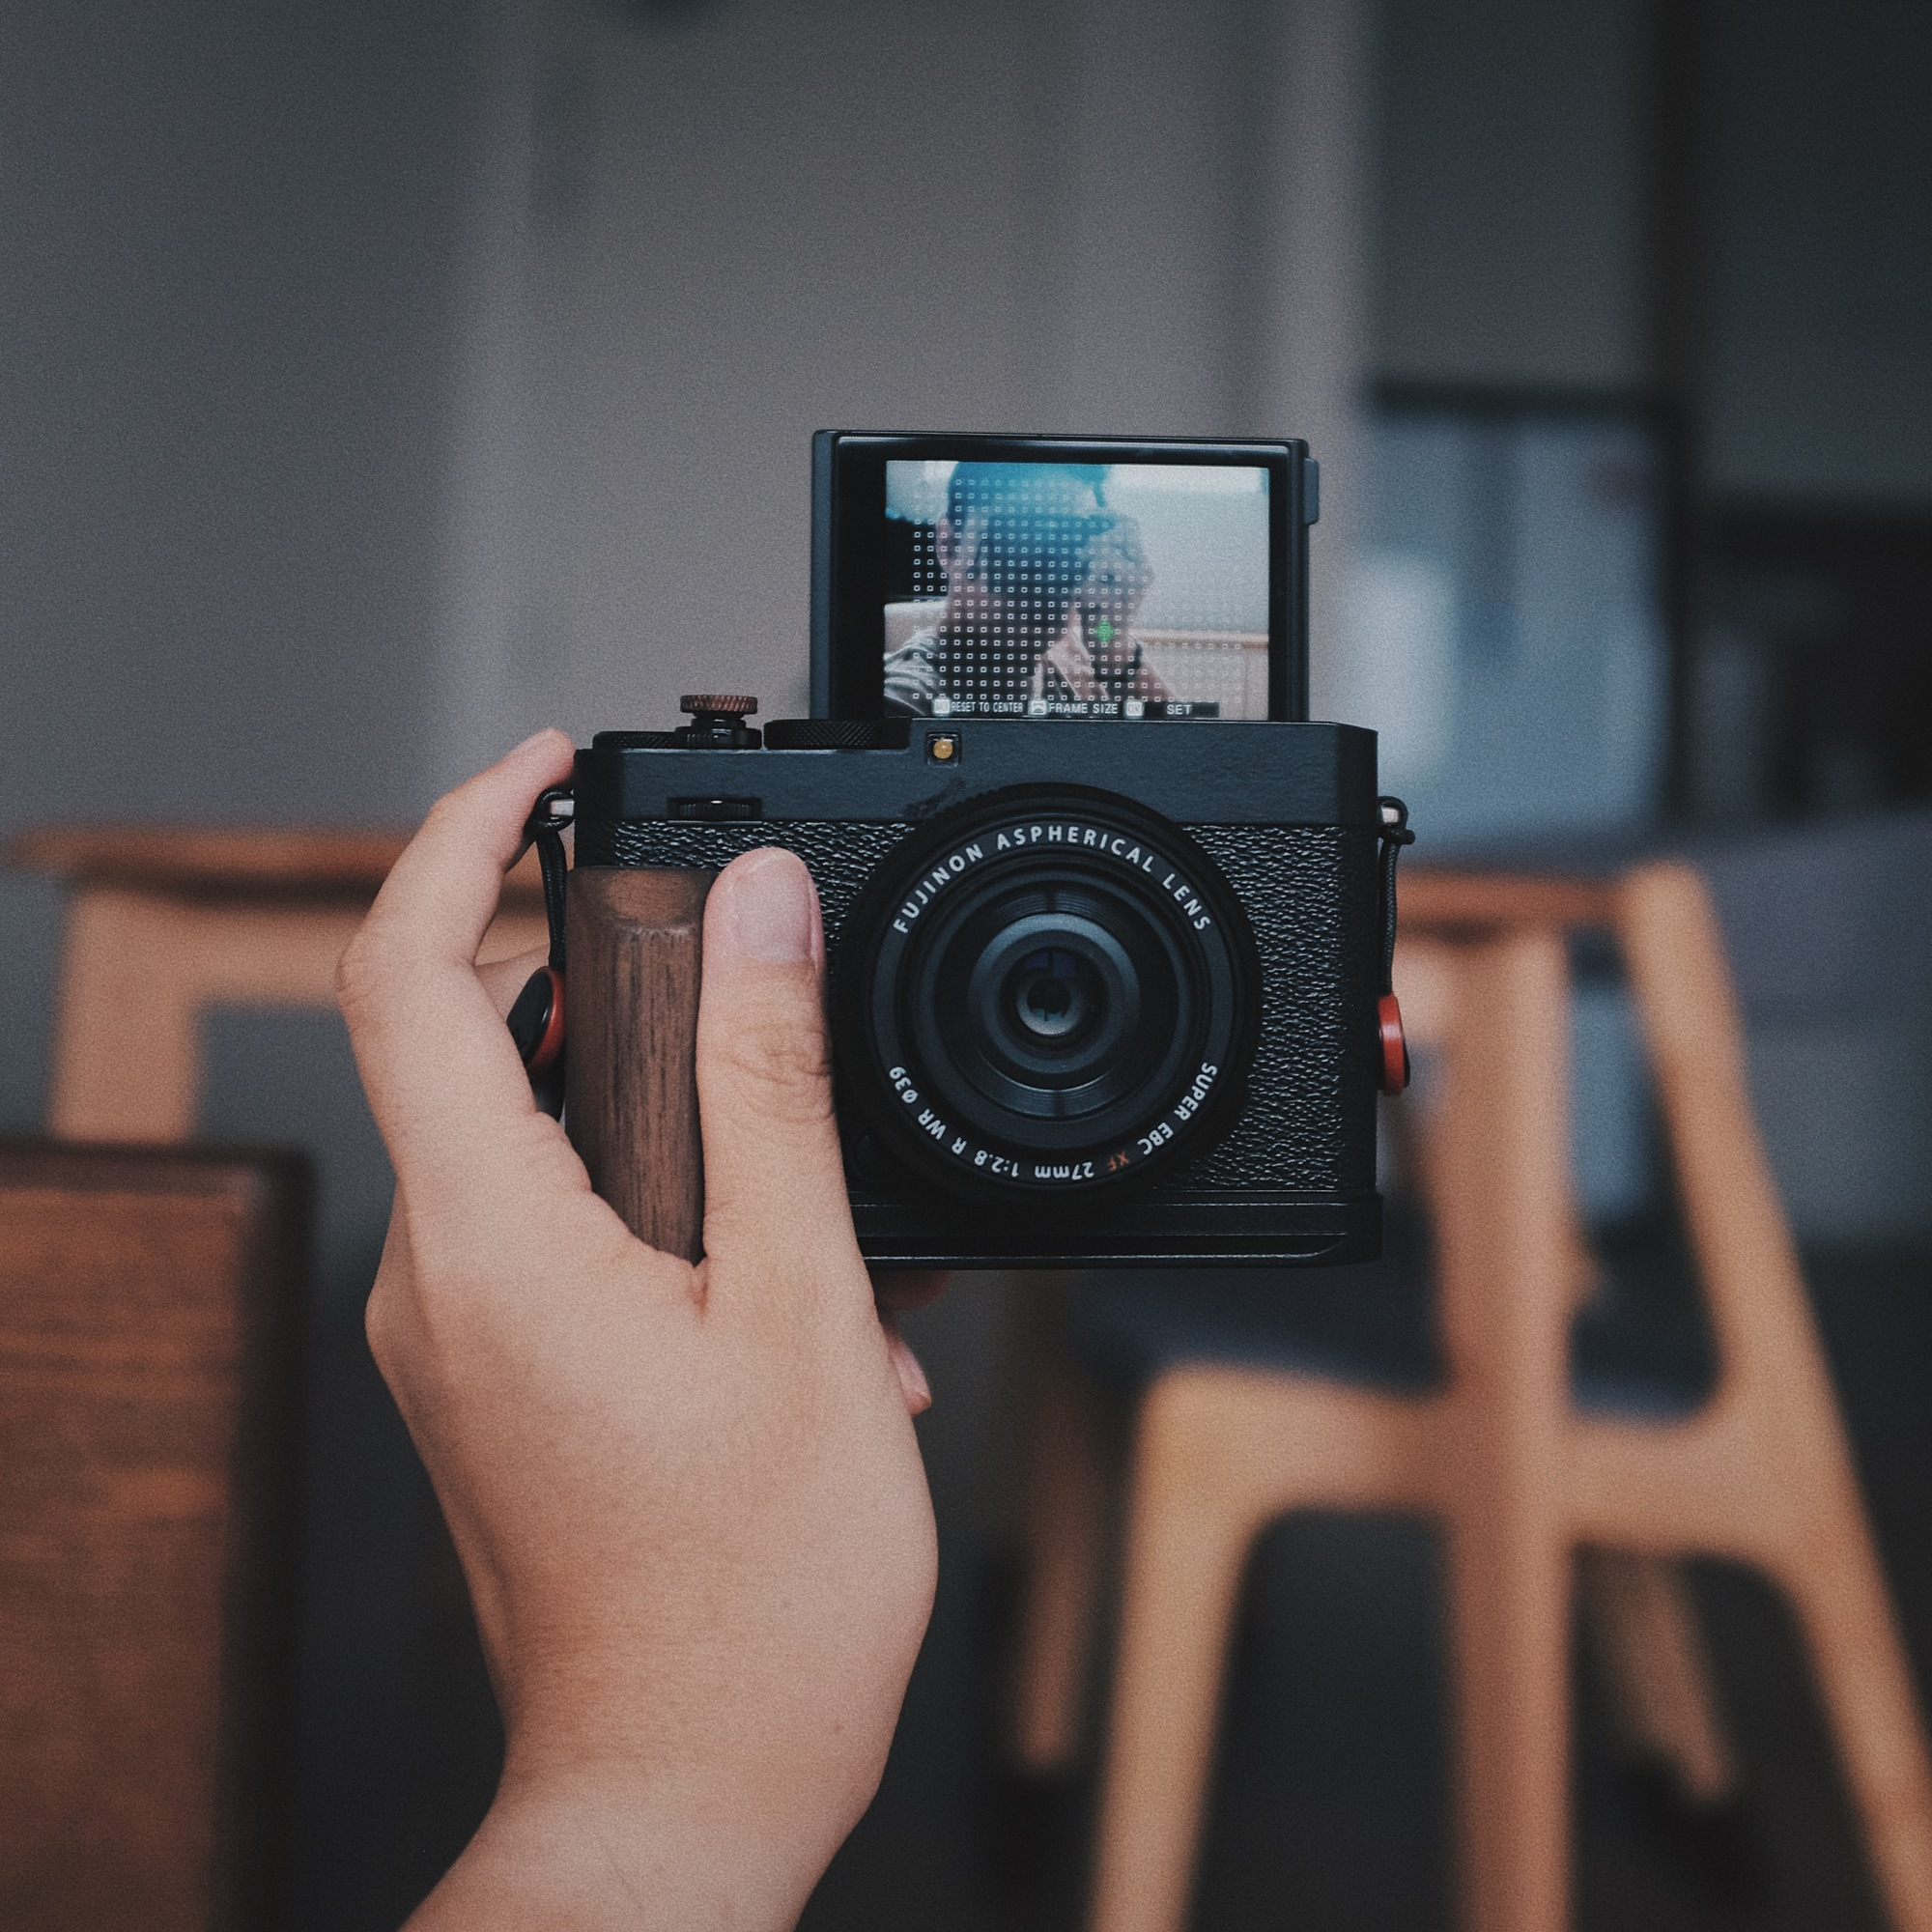
\includegraphics[width=\linewidth]{\envfinaldir/coverpic-prod.jpg}\par
            % \vskip 30pt
            \vfill

            \normalsize\rmfamily\scshape
            \copyright{} The Web Digest Project \hfill\large \envdatestr
        \end{center}
    \end{titlepage}
    % \restoregeometry
}
\newcommand{\simplehref}[1]{%
    \textcolor{blue!80!green}{\href{#1}{#1}}%
}
\renewcommand{\contentsname}{\center\Huge\sffamily\bfseries Contents\par\vskip 20pt}
\newcounter{ipartcounter}
\setcounter{ipartcounter}{0}
\newcommand{\ipart}[1]{
    % \vskip 20pt
    \clearpage
    \stepcounter{ipartcounter}
    \phantomsection
    \addcontentsline{toc}{chapter}{#1}
    % \begin{center}
    %     \Huge
    %     \sffamily\bfseries
    %     #1
    % \end{center}
    % \vskip 20pt plus 7pt
}
\newcounter{ichaptercounter}
\setcounter{ichaptercounter}{0}
\newcommand{\ichapter}[1]{
    % \vskip 20pt
    \clearpage
    \stepcounter{ichaptercounter}
    \phantomsection
    \addcontentsline{toc}{section}{\numberline{\arabic{ichaptercounter}}#1}
    \begin{center}
        \Huge
        \sffamily\bfseries
        #1
    \end{center}
    \vskip 20pt plus 7pt
}
\newcommand{\entrytitlefont}[1]{\subsection*{\raggedright\Large\sffamily\bfseries#1}}
\newcommand{\entryitemGeneric}[2]{
    % argv: title, url
    \parbox{\linewidth}{
        \entrytitlefont{#1}\par\vskip 5pt
        \footnotesize\ttfamily\mdseries
        \simplehref{#2}
    }\vskip 11pt plus 11pt minus 1pt
}
\newcommand{\entryitemGithub}[3]{
    % argv: title, url, desc
    \parbox{\linewidth}{
        \entrytitlefont{#1}\par\vskip 5pt
        \footnotesize\ttfamily\mdseries
        \simplehref{#2}\par\vskip 5pt
        \small\rmfamily\mdseries#3
    }\vskip 11pt plus 11pt minus 1pt
}
\newcommand{\entryitemAp}[3]{
    % argv: title, url, desc
    \parbox{\linewidth}{
        \entrytitlefont{#1}\par\vskip 5pt
        \footnotesize\ttfamily\mdseries
        \simplehref{#2}\par\vskip 5pt
        \small\rmfamily\mdseries#3
    }\vskip 11pt plus 11pt minus 1pt
}
\newcommand{\entryitemHackernews}[3]{
    % argv: title, hnurl, rawurl
    % \parbox{\linewidth}{
    %     \entrytitlefont{#1}\par\vskip 5pt
    %     \footnotesize\ttfamily\mdseries
    %     \simplehref{#3}\par
    %     \textcolor{black!50}{\href{#2}{#2}}
    % }\vskip 11pt plus 11pt minus 1pt
    \begin{minipage}{\linewidth}
            \entrytitlefont{#1}\par\vskip 5pt
            \footnotesize\ttfamily\mdseries
            \simplehref{#3}\par
            \textcolor{black!50}{\href{#2}{#2}}
    \end{minipage}\par\vskip 11pt plus 11pt minus 1pt
}







\begin{document}

\makeheader

\tableofcontents\clearpage




\ipart{Developers}
\ichapter{Hacker News}
\entryitemTwoLinks{Oxide's compensation model: how is it going?}{https://news.ycombinator.com/item?id=43862487}{https://oxide.computer/blog/oxides-compensation-model-how-is-it-going}

\entryitemTwoLinks{New Study: Waymo is reducing serious crashes and making streets safer}{https://news.ycombinator.com/item?id=43861828}{https://waymo.com/blog/2025/05/waymo-making-streets-safer-for-vru}

\entryitemTwoLinks{Dopamine signals when a fear can be forgotten}{https://news.ycombinator.com/item?id=43860726}{https://picower.mit.edu/news/dopamine-signals-when-fear-can-be-forgotten}

\entryitemTwoLinks{The Gang Has a Mid-Life Crisis}{https://news.ycombinator.com/item?id=43860696}{https://chris-martin.org/2025/the-gang-has-a-mid-life-crisis}

\entryitemTwoLinks{Arizona laptop farmer pleads guilty for funneling \$17M to Kim Jong Un}{https://news.ycombinator.com/item?id=43860207}{https://www.theregister.com/2025/02/12/arizona\_woman\_laptop\_farm\_guilty/}

\entryitemTwoLinks{Llasa: Llama-Based Speech Synthesis}{https://news.ycombinator.com/item?id=43860137}{https://llasatts.github.io/llasatts/}

\entryitemTwoLinks{Claude Integrations}{https://news.ycombinator.com/item?id=43859536}{https://www.anthropic.com/news/integrations}

\entryitemTwoLinks{Show HN: Roons – Mechanical Computer Kit}{https://news.ycombinator.com/item?id=43859464}{https://whomtech.com/show-hn/}

\entryitemTwoLinks{Redis is open source again}{https://news.ycombinator.com/item?id=43859446}{https://antirez.com/news/151}

\entryitemTwoLinks{The term "vegetative electron microscopy" keeps showing up in scientific papers}{https://news.ycombinator.com/item?id=43858655}{https://www.sciencealert.com/a-strange-phrase-keeps-turning-up-in-scientific-papers-but-why}

\entryitemTwoLinks{Starting July 1, academic publishers can't paywall NIH-funded research}{https://news.ycombinator.com/item?id=43858568}{https://www.nih.gov/about-nih/who-we-are/nih-director/statements/accelerating-access-research-results-new-implementation-date-2024-nih-public-access-policy}

\entryitemTwoLinks{We identified a North Korean hacker who tried to get a job}{https://news.ycombinator.com/item?id=43858462}{https://blog.kraken.com/news/how-we-identified-a-north-korean-hacker}

\entryitemTwoLinks{RFK Jr. rejects cornerstone of health science: Germ theory}{https://news.ycombinator.com/item?id=43857903}{https://arstechnica.com/health/2025/04/rfk-jr-s-anti-vaccine-stance-is-rooted-in-a-disbelief-in-germ-theory/}

\entryitemTwoLinks{Vanguard 50-year anniversary CEO letter}{https://news.ycombinator.com/item?id=43857862}{https://corporate.vanguard.com/content/corporatesite/us/en/corp/articles/of-investor-by-investor-for-investor-since-1975.html}

\entryitemTwoLinks{International Workers' Day}{https://news.ycombinator.com/item?id=43856803}{https://en.wikipedia.org/wiki/International\_Workers\%27\_Day}

\entryitemTwoLinks{Linkwarden: FOSS self-hostable bookmarking with AI-tagging and page archival}{https://news.ycombinator.com/item?id=43856801}{https://linkwarden.app/}

\entryitemTwoLinks{The Brief Origins of May Day}{https://news.ycombinator.com/item?id=43856798}{https://archive.iww.org/history/library/misc/origins\_of\_mayday/}

\entryitemTwoLinks{Judge rules Apple executive lied under oath, makes criminal contempt referral}{https://news.ycombinator.com/item?id=43856795}{https://www.thebignewsletter.com/p/judge-rules-apple-executive-lied}

\entryitemTwoLinks{Trust Me, I'm Local: Chrome Extensions, MCP, and the Sandbox Escape}{https://news.ycombinator.com/item?id=43856656}{https://blog.extensiontotal.com/trust-me-im-local-chrome-extensions-mcp-and-the-sandbox-escape-1875a0ee4823}

\entryitemTwoLinks{Running Qwen3 on your macbook, using MLX, to vibe code for free}{https://news.ycombinator.com/item?id=43856489}{https://localforge.dev/blog/running-qwen3-macbook-mlx}\ichapter{Phoronix}
\entryitemGeneric{\hskip 0pt{}Plasma LTS Releases Being Discontinued, Better KDE Telemetry Like Valve's Steam Survey}{https://www.phoronix.com/news/KDE-Plasma-Graz-Sprint}

\entryitemGeneric{\hskip 0pt{}Redis 8.0 Released: Now Tri-Licensed With AGPLv3}{https://www.phoronix.com/news/Redis-8.0-Goes-AGPLv3}

\entryitemGeneric{\hskip 0pt{}Ubuntu 25.10 "Questing Quokka" Opens For Development}{https://www.phoronix.com/news/Ubuntu-25.10-Development-Start}

\entryitemGeneric{\hskip 0pt{}GCC 15 Compiler Demonstrating Measurable Performance Gains For AMD EPYC Turin}{https://www.phoronix.com/review/gcc15-amd-epyc-turin}

\entryitemGeneric{\hskip 0pt{}Kcompressd Proposed For Accelerated Memory Compression On Linux}{https://www.phoronix.com/news/Linux-Kcompressd-Memory}

\entryitemGeneric{\hskip 0pt{}Patch Posted For Addressing The AMD CPU Performance Regression On Linux 6.15}{https://www.phoronix.com/news/Linux-6.15-Patch-For-AMD}

\entryitemGeneric{\hskip 0pt{}LibreOffice Begins Landing Zstd Integration}{https://www.phoronix.com/news/LibreOffice-Landing-Zstd}

\entryitemGeneric{\hskip 0pt{}Framework 13 With Strix Point, Cheap RISC-V \& Linux Kernel Happenings Topped April}{https://www.phoronix.com/news/April-2025-Highlights}

\entryitemGeneric{\hskip 0pt{}Sculpt OS 25.04 Released With Support For Intel Meteor Lake}{https://www.phoronix.com/news/Sculpt-OS-25.04}\ichapter{Dribbble}
\entryitemGeneric{\hskip 0pt{}South Africa}{https://dribbble.com/shots/25967008-South-Africa}

\entryitemGeneric{\hskip 0pt{}Startup UI UX Design, User Interface Experience for Tempest}{https://dribbble.com/shots/25960670-Startup-UI-UX-Design-User-Interface-Experience-for-Tempest}

\entryitemGeneric{\hskip 0pt{}NEW YORK}{https://dribbble.com/shots/25962578-NEW-YORK}

\entryitemGeneric{\hskip 0pt{}Spin Twin // Website}{https://dribbble.com/shots/25960774-Spin-Twin-Website}

\entryitemGeneric{\hskip 0pt{}Aura - Brand System}{https://dribbble.com/shots/25962395-Aura-Brand-System}

\entryitemGeneric{\hskip 0pt{}New Logo Collection}{https://dribbble.com/shots/25960892-New-Logo-Collection}

\entryitemGeneric{\hskip 0pt{}AI Brand Mascot for Sports Tech}{https://dribbble.com/shots/25962416-AI-Brand-Mascot-for-Sports-Tech}

\entryitemGeneric{\hskip 0pt{}Landing Page DeFi Design}{https://dribbble.com/shots/25961311-Landing-Page-DeFi-Design}

\entryitemGeneric{\hskip 0pt{}Helio}{https://dribbble.com/shots/25955551-Helio}

\entryitemGeneric{\hskip 0pt{}R}{https://dribbble.com/shots/25954740-R}

\entryitemGeneric{\hskip 0pt{}Crypto Exchange Mobile UI}{https://dribbble.com/shots/25955808-Crypto-Exchange-Mobile-UI}

\entryitemGeneric{\hskip 0pt{}Letter F Logos}{https://dribbble.com/shots/25956899-Letter-F-Logos}

\entryitemGeneric{\hskip 0pt{}Sellin UI Kit on UI8 download}{https://dribbble.com/shots/25948738-Sellin-UI-Kit-on-UI8-download}

\entryitemGeneric{\hskip 0pt{}Novure - Fashion Online Store e-Commerce Landing Page Website}{https://dribbble.com/shots/25959299-Novure-Fashion-Online-Store-e-Commerce-Landing-Page-Website}

\entryitemGeneric{\hskip 0pt{}Core 2.0 – Dashboard Builder}{https://dribbble.com/shots/25956157-Core-2-0-Dashboard-Builder}

\entryitemGeneric{\hskip 0pt{}Finergy UIkit on UI8}{https://dribbble.com/shots/25948707-Finergy-UIkit-on-UI8}

\entryitemGeneric{\hskip 0pt{}Clint}{https://dribbble.com/shots/25947599-Clint}

\entryitemGeneric{\hskip 0pt{}Fat Cat Movie Night}{https://dribbble.com/shots/25947610-Fat-Cat-Movie-Night}

\entryitemGeneric{\hskip 0pt{}Tallybreeze Logo Design - Accounting Automation for Property}{https://dribbble.com/shots/25946704-Tallybreeze-Logo-Design-Accounting-Automation-for-Property}

\entryitemGeneric{\hskip 0pt{}Maybelline // 3D Promo Animation}{https://dribbble.com/shots/25946191-Maybelline-3D-Promo-Animation}

\entryitemGeneric{\hskip 0pt{}Progressive RV Insurance Print Ads}{https://dribbble.com/shots/25948535-Progressive-RV-Insurance-Print-Ads}

\entryitemGeneric{\hskip 0pt{}New Personal Website}{https://dribbble.com/shots/25947555-New-Personal-Website}

\entryitemGeneric{\hskip 0pt{}Onboarding screen collection}{https://dribbble.com/shots/25943700-Onboarding-screen-collection}

\entryitemGeneric{\hskip 0pt{}Rhino Dragon}{https://dribbble.com/shots/25945050-Rhino-Dragon}


\ipart{Developers~~~~(zh-Hans)}
\ichapter{Solidot}
\entryitemGeneric{\hskip 0pt{}因经济动荡 LWN 考虑涨价}{https://www.solidot.org/story?sid=81193}

\entryitemGeneric{\hskip 0pt{}撞击月球产生的碎片四分之一掉落到地球}{https://www.solidot.org/story?sid=81192}

\entryitemGeneric{\hskip 0pt{}Google 称政府更频繁的使用 0day}{https://www.solidot.org/story?sid=81191}

\entryitemGeneric{\hskip 0pt{}Firefox 138 释出,标签组正式推出}{https://www.solidot.org/story?sid=81190}

\entryitemGeneric{\hskip 0pt{}芬兰议会通过限制中小学生使用手机的法律}{https://www.solidot.org/story?sid=81189}

\entryitemGeneric{\hskip 0pt{}黄金可能来自磁星}{https://www.solidot.org/story?sid=81188}

\entryitemGeneric{\hskip 0pt{}LG 将于 6 月底关闭智能手机更新服务}{https://www.solidot.org/story?sid=81187}

\entryitemGeneric{\hskip 0pt{}Google Play 应用数量减少 47\%}{https://www.solidot.org/story?sid=81186}

\entryitemGeneric{\hskip 0pt{}前苏联失败的金星探测器即将坠落回地面}{https://www.solidot.org/story?sid=81185}

\entryitemGeneric{\hskip 0pt{}入侵餐厅菜单软件修改过敏信息的前迪士尼员工被判三年}{https://www.solidot.org/story?sid=81184}

\entryitemGeneric{\hskip 0pt{}西班牙和葡萄牙大规模停电原因是极端气温变化}{https://www.solidot.org/story?sid=81183}

\entryitemGeneric{\hskip 0pt{}因长时间盯着屏幕年轻一代出现干眼症}{https://www.solidot.org/story?sid=81182}

\entryitemGeneric{\hskip 0pt{}亚马逊将在商品价格中显示关税,白宫谴责}{https://www.solidot.org/story?sid=81181}

\entryitemGeneric{\hskip 0pt{}经济学家发现生成式 AI 没有取代工作或影响薪水}{https://www.solidot.org/story?sid=81180}

\entryitemGeneric{\hskip 0pt{}物质使用通过不同分子途径加速大脑老化}{https://www.solidot.org/story?sid=81179}

\entryitemGeneric{\hskip 0pt{}天然补充剂 Cel System 或有助于延缓衰老}{https://www.solidot.org/story?sid=81178}

\entryitemGeneric{\hskip 0pt{}价值 3.307 亿美元比特币的疑似被盗}{https://www.solidot.org/story?sid=81177}

\entryitemGeneric{\hskip 0pt{}汽车订阅功能增加司机被政府监视风险}{https://www.solidot.org/story?sid=81176}

\entryitemGeneric{\hskip 0pt{}阿里发布新开源权重模型 Qwen3}{https://www.solidot.org/story?sid=81175}

\entryitemGeneric{\hskip 0pt{}亚马逊发射首批互联网卫星}{https://www.solidot.org/story?sid=81174}\ichapter{V2EX}
\entryitemGeneric{\hskip 0pt{}[前端开发] 因为玩了《歧路旅人 II》,写了一个像素编辑器,欢迎大家体验。}{https://www.v2ex.com/t/1129362}

\entryitemGeneric{\hskip 0pt{}[Android] RedmiNote12turbo(marble)刷写 Aospa-Anroid15 的问题}{https://www.v2ex.com/t/1129361}

\entryitemGeneric{\hskip 0pt{}[杭州] 杭州怎么才能认识牛人啊?}{https://www.v2ex.com/t/1129360}

\entryitemGeneric{\hskip 0pt{}[硬件] 购买的海信 G9 到货了,说说问题并喷一下海信。}{https://www.v2ex.com/t/1129359}

\entryitemGeneric{\hskip 0pt{}[硬件] miniled 的效果真的好惊艳啊🤣}{https://www.v2ex.com/t/1129358}

\entryitemGeneric{\hskip 0pt{}[游戏] 有没有老哥和朋友玩过双人成行的}{https://www.v2ex.com/t/1129357}

\entryitemGeneric{\hskip 0pt{}[问与答] SeLinux 简直让人崩溃!}{https://www.v2ex.com/t/1129356}

\entryitemGeneric{\hskip 0pt{}[分享创造] 做了个颜值打分产品}{https://www.v2ex.com/t/1129355}

\entryitemGeneric{\hskip 0pt{}[分享发现] Twitter 去客户端广告}{https://www.v2ex.com/t/1129354}

\entryitemGeneric{\hskip 0pt{}[问与答] 人在菲律宾,有没有什么值得注册的?}{https://www.v2ex.com/t/1129352}

\entryitemGeneric{\hskip 0pt{}[问与答] win 远程总提示``登录到被阻止的会话''如何解决}{https://www.v2ex.com/t/1129350}

\entryitemGeneric{\hskip 0pt{}[分享发现] 含 AFF,infini 虚拟 u 卡降费率到 0.8\%了}{https://www.v2ex.com/t/1129349}

\entryitemGeneric{\hskip 0pt{}[产品经理茶话会] 产品变为全栈?}{https://www.v2ex.com/t/1129348}

\entryitemGeneric{\hskip 0pt{}[随想] 错误的事情,坚持下去,就会付出惨重的代价!}{https://www.v2ex.com/t/1129347}

\entryitemGeneric{\hskip 0pt{}[问与答] 新闻报道,永辉超市收银出现反向抹零(7.96 元计 8 元)。通告整改为去尾法(7.96 元计 7.9 元)}{https://www.v2ex.com/t/1129346}

\entryitemGeneric{\hskip 0pt{}[软件] Linux Debian 有什么好用的脑图软件?}{https://www.v2ex.com/t/1129345}

\entryitemGeneric{\hskip 0pt{}[推广] 4Zapi 一站式 AI API 中转服务,支持 GPT/Grok/Gemini 等主流模型}{https://www.v2ex.com/t/1129344}

\entryitemGeneric{\hskip 0pt{}[iPhone] 巨魔你们都用什么 超级好用的 插件? 除了常用的那几个 什么通话录音、虚拟定位什么的}{https://www.v2ex.com/t/1129343}

\entryitemGeneric{\hskip 0pt{}[分享发现] 由排序算法想到的}{https://www.v2ex.com/t/1129342}

\entryitemGeneric{\hskip 0pt{}[问与答] 一次性手套居然也不卫生?}{https://www.v2ex.com/t/1129340}

\entryitemGeneric{\hskip 0pt{}[MacBook Pro] M1-Max 的 E-Core 长期接近满载导致操作卡顿,该淘汰了吗?}{https://www.v2ex.com/t/1129339}

\entryitemGeneric{\hskip 0pt{}[问与答] 请教,有大佬知道如何在国内使用 WhatsApp 吗?}{https://www.v2ex.com/t/1129337}

\entryitemGeneric{\hskip 0pt{}[程序员] 分享一个 OCR 软件(基于 LLM 可识别 Latex)}{https://www.v2ex.com/t/1129336}

\entryitemGeneric{\hskip 0pt{}[程序员] 订阅年费 Cursor,取消 Claude 订阅}{https://www.v2ex.com/t/1129335}

\entryitemGeneric{\hskip 0pt{}[硬件] 罗技 anywhere 3 右键彻底废了,换微动也没反应!}{https://www.v2ex.com/t/1129334}

\entryitemGeneric{\hskip 0pt{}[生活] 请问现在去香港开汇丰 one 门槛高吗?}{https://www.v2ex.com/t/1129333}

\entryitemGeneric{\hskip 0pt{}[分享创造] 发现一个神奇的 DEMO HUB(或者也有可能是原型坟场?)}{https://www.v2ex.com/t/1129332}

\entryitemGeneric{\hskip 0pt{}[iPhone] iPhone 16 到底支持不支持 4800W 像素,为什么所有人都说支持,实际不支持。}{https://www.v2ex.com/t/1129331}

\entryitemGeneric{\hskip 0pt{}[买买买] 分享张一号店会员的副卡,可以免一次运费}{https://www.v2ex.com/t/1129330}

\entryitemGeneric{\hskip 0pt{}[iPhone] 你们用巨魔多开 app 有被封过号吗 比如闲鱼 APP}{https://www.v2ex.com/t/1129329}

\entryitemGeneric{\hskip 0pt{}[问与答] 请问一下老哥们,纯小白,旱鸭子,想学习游泳,是看 B 站视频自学好,还是报班好?}{https://www.v2ex.com/t/1129327}

\entryitemGeneric{\hskip 0pt{}[宽带症候群] 上海联通 5 月套餐内容增容价格不变}{https://www.v2ex.com/t/1129326}

\entryitemGeneric{\hskip 0pt{}[生活] [记录]-2025-05-01 在看《天国王朝》}{https://www.v2ex.com/t/1129325}

\entryitemGeneric{\hskip 0pt{}[分享创造] [xim+]: 最新 gcc15.1.0 发布, 一键从源码构建 -- c++23 import std 启动}{https://www.v2ex.com/t/1129324}

\entryitemGeneric{\hskip 0pt{}[物联网] 想搞一张飞天诚信(ftsafe)的指纹卡(或者同类型卡),请问哪里可以购买?}{https://www.v2ex.com/t/1129323}

\entryitemGeneric{\hskip 0pt{}[问与答] 生成了个邀请码给朋友,但是他回复帖子直接回转到首页,再次进入回复的帖子刷新后也看不到回复,请问是怎么回事?}{https://www.v2ex.com/t/1129322}

\entryitemGeneric{\hskip 0pt{}[问与答] 自己创业负债 200 万,不知道怎么翻身}{https://www.v2ex.com/t/1129321}

\entryitemGeneric{\hskip 0pt{}[分享创造] 开发了个图片 AI 增强的应用,自己部署了模型来调用的}{https://www.v2ex.com/t/1129320}

\entryitemGeneric{\hskip 0pt{}[Linux] 有没有办法在 lxc 特权容器中用普通用户运行 podman?}{https://www.v2ex.com/t/1129319}

\entryitemGeneric{\hskip 0pt{}[iPhone] 高版本系统备份恢复到低版本 手机会有很多莫名其妙的问题、你们遇到过吗}{https://www.v2ex.com/t/1129318}

\entryitemGeneric{\hskip 0pt{}[问与答] 手机的 5G 有没有可能在闲置时,作为微型基站转发数据?}{https://www.v2ex.com/t/1129317}

\entryitemGeneric{\hskip 0pt{}[推广] 还没开始,尴尬住了。。}{https://www.v2ex.com/t/1129316}

\entryitemGeneric{\hskip 0pt{}[问与答] 求推荐初一初二线上课程}{https://www.v2ex.com/t/1129315}

\entryitemGeneric{\hskip 0pt{}[分享创造] 用 Manus 又做了一个``小废物''还弄了一个小彩蛋 0(O\_o)0}{https://www.v2ex.com/t/1129314}

\entryitemGeneric{\hskip 0pt{}[NAS] emby 怎么鼠标悬停在影片上自动播放预览,类似 p 站那样}{https://www.v2ex.com/t/1129311}

\entryitemGeneric{\hskip 0pt{}[问与答] 新加坡 rustdesk 上海, 71ping 算极佳了不.}{https://www.v2ex.com/t/1129307}

\entryitemGeneric{\hskip 0pt{}[Apple] HomePod mini 是不是对 5GWi-Fi 很不友好}{https://www.v2ex.com/t/1129306}

\entryitemGeneric{\hskip 0pt{}[问与答] 关于 Easytier 组网突然失联的疑问}{https://www.v2ex.com/t/1129305}

\entryitemGeneric{\hskip 0pt{}[酷工作] 找个远程前端}{https://www.v2ex.com/t/1129304}

\entryitemGeneric{\hskip 0pt{}[加密货币] 失业程序员,回家养鸡。不甘现状,想挣钱。}{https://www.v2ex.com/t/1129301}


\ipart{Generic News}
\ichapter{AP News}
\entryitemWithDescription{\hskip 0pt{}Over 2 million Ninja-branded pressure cookers are recalled after reports of serious burn injuries}{https://apnews.com/article/4d9a56f0a4ec169fd8832d072a78e512}{}

\entryitemWithDescription{\hskip 0pt{}Australian locals rescue great white shark stranded in shallow water}{https://apnews.com/article/323cc74c32380c3b71a2dae70dbbf387}{}

\entryitemWithDescription{\hskip 0pt{}UK counterterror police say they will investigate comments by Irish rap group Kneecap}{https://apnews.com/article/3cc86cf249c366554dee3cf5dd498fdc}{}

\entryitemWithDescription{\hskip 0pt{}Man who fell from 21-foot Clemente Wall at PNC Park during Pirates game in critical condition}{https://apnews.com/article/88128fb881551cf9fb343f2a64f60aa0}{}

\entryitemWithDescription{\hskip 0pt{}UNC's Belichick defends Hudson as `doing her job' after interjecting during CBS interview}{https://apnews.com/article/444939d933e4f92f280f62ba6b193de1}{}

\entryitemWithDescription{\hskip 0pt{}Giannis Antetokounmpo enters this offseason with a big question awaiting him. Stay or go?}{https://apnews.com/article/66bafbefa40bb09943a3d60b23a206f0}{}

\entryitemWithDescription{\hskip 0pt{}The home of Elon Musk's SpaceX could become an official Texas city called Starbase}{https://apnews.com/article/f17e2980756e9129b416022729bd67ac}{}

\entryitemWithDescription{\hskip 0pt{}NFL fines Falcons and defensive coordinator Jeff Ulbrich following prank call to Shedeur Sanders}{https://apnews.com/article/be7efb4084d4deb4821b95cb43919e4d}{}

\entryitemWithDescription{\hskip 0pt{}Barcelona and Inter Milan draw 3-3 in thrilling first leg of their Champions League semifinal}{https://apnews.com/article/822523780ac99a58d28b1a1dfea94ffd}{}

\entryitemWithDescription{\hskip 0pt{}A town refuses to give up the school's Native American mascot — and gets Trump's support}{https://apnews.com/article/fc750c700733949805afd8266c69a975}{}

\entryitemWithDescription{\hskip 0pt{}The women of `Andor' see their roles get bigger, and go deeper, in Season 2}{https://apnews.com/article/73a018cbe799ae1e01bb31362243b992}{}

\entryitemWithDescription{\hskip 0pt{}A man airlifted from Japan's Mount Fuji returns to the slope days later and is rescued again}{https://apnews.com/article/bc1fcc11150238dee96370697944991b}{}

\entryitemWithDescription{\hskip 0pt{}`Sinners' bites off a phenomenal second weekend as a 20-year-old Star Wars movie takes second place}{https://apnews.com/article/77acfe0d0f005a39d72f2de7d4c4748a}{}






\clearpage
\leavevmode\vfill
\footnotesize

Copyright \copyright{} 2023-2025 Neruthes and other contributors.

This document is published with CC BY-NC-ND 4.0 license.

The entries listed in this newsletter may be copyrighted by their respective creators.

This newsletter is generated by the Web Digest project.

The newsletters are also delivered via Telegram channel \CJKunderline{\href{https://t.me/webdigestchannel}{https://t.me/webdigestchannel}}.\\
RSS feed is available at \CJKunderline{\href{https://webdigest.pages.dev/rss.xml}{https://webdigest.pages.dev/rss.xml}}.

This newsletter is available in PDF at
\CJKunderline{\href{https://webdigest.pages.dev/}{https://webdigest.pages.dev/}}.

The source code being used to generate this newsletter is available at\\
\CJKunderline{\href{https://github.com/neruthes/webdigest}{https://github.com/neruthes/webdigest}}.

This newsletter is also available in
\CJKunderline{\href{http://webdigest.pages.dev/readhtml/\envyear/WebDigest-20250502.html}{HTML}} and
\CJKunderline{\href{https://github.com/neruthes/webdigest/blob/master/markdown/\envyear/WebDigest-20250502.md}{Markdown}}.


\coverpic{https://unsplash.com/photos/a-cowboy-sits-on-his-horse-in-the-desert-9nqNQLfn5B4}{Diego PH}


\end{document}
